%  TESINA / PROYECTO DE INNOVACIÓN Y/O MEJORA - Formato SENATI

% ------------------------------------------

\documentclass[12pt,a4paper]{report}

% ---------- Idioma y codificación ----------
\usepackage[utf8]{inputenc}
\usepackage[T1]{fontenc}
\usepackage[spanish,es-tabla]{babel}
\usepackage{float}
\decimalpoint

% ---------- Tipografía estilo Times ----------
\usepackage{mathptmx}

% ---------- Márgenes tipo APA (2.5 cm / 1 pulgada) ----------
\usepackage[a4paper,margin=2.5cm]{geometry}

% ---------- Interlineado ----------
\usepackage{setspace}
\onehalfspacing
%doble espacio estricto (APA puro)esta:
% \doublespacing

% ---------- Encabezado y pie de página ----------
\usepackage{fancyhdr}
\pagestyle{fancy}
\setlength{\headheight}{14.5pt}
\fancyhf{}
\fancyhead[L]{Sistema web de gestión tributaria predial con Machine Learning} 
\fancyhead[R]{\thepage}
\renewcommand{\headrulewidth}{0.4pt}
% Las primeras páginas de capítulo usan el estilo 'plain': que conserven encabezado y número
\fancypagestyle{plain}{%
  \fancyhf{}
  \fancyhead[L]{Sistema web de gestión tributaria predial con Machine Learning}
  \fancyhead[R]{\thepage}
  \renewcommand{\headrulewidth}{0.4pt}
}

% ---------- Otros paquetes útiles ----------
\usepackage{graphicx}
\usepackage{caption}
\usepackage{booktabs}
\usepackage{longtable}
\usepackage{enumitem}
\usepackage{amsmath,amssymb}
\usepackage[hidelinks]{hyperref}
\usepackage{csquotes}
\usepackage[
  backend=biber,
  style=apa,
  sorting=nyt
]{biblatex}
\DeclareLanguageMapping{spanish}{spanish-apa} % APA en español ("y", "s.f.", etc.)
\addbibresource{referencias.bib}

\graphicspath{{imagenes/}}

% Inserta la imagen si existe; si no, muestra un recuadro marcador (no rompe la compilación)
\newcommand{\imgopt}[2]{%
  \IfFileExists{imagenes/#2}{\includegraphics[width=#1\textwidth]{#2}}%
  {\fbox{\parbox[c][4cm][c]{0.6\textwidth}{\centering\textit{[Insertar imagen: \detokenize{#2}]}}}}%
}

% ---------- Numeración de capítulos tipo "1.1.1." ----------
\setcounter{secnumdepth}{4}
\setcounter{tocdepth}{4}

% ---------- Numeración de Tablas/Figuras "Tabla 1", "Figura 1" (sin capítulo) ----------
\usepackage{chngcntr}
\counterwithout{table}{chapter}   % que no se reinicien en cada capítulo
\counterwithout{figure}{chapter}
\renewcommand{\thetable}{\arabic{table}}
\renewcommand{\thefigure}{\arabic{figure}}

\title{Sistema web de gestión tributaria predial con Machine Learning}
\author{[Tus nombres]}
\date{[Mes y año]}

\begin{document}


% ---------- CARÁTULA---------- 

\begin{titlepage}
\centering

\includegraphics[width=0.5\textwidth]{logo_senati.png}\par
\vspace{0.5cm}

{\large SERVICIO NACIONAL DE ADIESTRAMIENTO EN TRABAJO INDUSTRIAL\par}
\vspace{0.2cm}
{\large\bfseries DIRECCIÓN ZONAL: LIMA -- CALLAO\par}
\vspace{0.2cm}
{\large ESCUELA DE TECNOLOGÍA DE LA INFORMACIÓN\par}
\vspace{0.2cm}
{\large CFP LUIS CÁCERES GRAZIANI\par}
\vspace{0.2cm}
{\large\bfseries INGENIERÍA DE SOFTWARE CON INTELIGENCIA ARTIFICIAL\par}
\vspace{0.2cm}
{\large Proyecto de Innovación y/o Mejora\par}
\vspace{0.2cm}
{\large Nivel Profesional Técnico/ Técnico Operativo\par}
\vspace{1.5cm}
% sad
{\Large\bfseries ``IMPLEMENTACIÓN DE UN SISTEMA WEB DE GESTIÓN TRIBUTARIA PREDIAL PARA OPTIMIZAR LA COBRANZA Y ESTIMAR EL RIESGO DE MOROSIDAD USANDO MACHINE LEARNING''\par}
\vspace{1.5cm}

{\bfseries Autores:\par}
\vspace{0.2cm}
{\large Renzo Alexis Pérez Gonzales\par}
{\large Xavier Eulices Gerdez Villalobos\par}
\vspace{1cm}

{\bfseries Asesor:\par}
\vspace{0.2cm}
{\large Mg. José Armando Tiznado Ubillus\par}
\vfill

{\bfseries Lima -- Callao\par}
\vspace{0.2cm}
{\bfseries 2026\par}
\end{titlepage}

\pagenumbering{arabic}


% ----------AGRADECIMIENTO----------

\chapter*{Agradecimiento}
\addcontentsline{toc}{chapter}{Agradecimiento}

En esta ocasión, mediante el presente trabajo quiero dedicar unas palabras a todas esas personas que me apoyaron y nunca me dejaron solo durante este proceso, ya que sin ellos nada de esto habría sido posible.
En primer lugar, agradezco a mis padres por su guía y motivación constante. Mis profesores, que me compartieron todo su conocimiento y me enseñaron la pasión por la tecnología. Mi hermanita, que siempre creyó en mí y nunca dudo de mis habilidades. Mis amigos, que me mantenían siempre feliz y sonriente.



% ----------DEDICATORIA----------
\chapter*{Dedicatoria}
\addcontentsline{toc}{chapter}{Dedicatoria}

A mi familia, que fue el pilar de mi formación y me apoyaron incondicionalmente desde el día 1, gracias por todo el sacrificio y por todo el cariño que me han dado siempre.

A mis profesores, por guiarme y hacer posible el crecimiento tanto personal como profesional que he conseguido.
A mí mismo, por no rendirme en el camino, por mantener la misma ilusión y las mismas ganas de aprender y de crecer.


% ----------RESUMEN----------
\chapter*{Resumen}
\addcontentsline{toc}{chapter}{Resumen}

El presente proyecto tiene como finalidad el desarrollo de un sistema informático web para la Municipalidad de San Bartolo, orientado a reemplazar el software de gestión municipal actualmente en uso, el cual fue desarrollado en Visual FoxPro 9 como una aplicación de escritorio local dependiente de un servidor físico. Esta dependencia limita la flexibilidad operativa de la institución, restringiendo el acceso al sistema únicamente a los equipos conectados a dicha infraestructura y dificultando su mantenimiento y escalabilidad a largo plazo.

Ante esta problemática, se propone la migración del sistema hacia una arquitectura web, que permita a los funcionarios municipales acceder a la plataforma desde cualquier ubicación con conexión a internet, eliminando la dependencia de un servidor local. El nuevo sistema conservará y optimizará las funcionalidades principales del software existente, entre las cuales se encuentran el registro de personas y propietarios, la gestión de propiedades, el procesamiento de transferencias de propiedad por concepto de venta, la baja de propiedades y el registro de propiedades heredadas, procesos característicos de la gestión catastral municipal.

La metodología de desarrollo contempla, en una primera etapa, el acceso y exploración del sistema actual con el objetivo de identificar de manera detallada sus funcionalidades, con el propósito de replicarlas e incorporar mejoras tanto a nivel tecnológico como de experiencia de usuario. El desarrollo se inicia con la implementación del módulo de autenticación (login), componente fundamental al tratarse de un sistema web que requiere control de acceso mediante usuario y contraseña, gestionado mediante tokens JWT y contraseñas cifradas con bcrypt.

Para la construcción del sistema se ha definido un stack tecnológico compuesto por Node.js con el framework NestJS y TypeScript para el desarrollo del backend, React junto con Tailwind CSS y Vite para la interfaz de usuario, y PostgreSQL con Prisma ORM como sistema gestor de base de datos relacional. Esta selección responde a criterios de escalabilidad, mantenibilidad del código y compatibilidad con el equipo de desarrollo.

Asimismo, el proyecto incorpora un modelo de Machine Learning que estima el riesgo de morosidad de los contribuyentes a partir del historial de pagos y deudas, con el fin de priorizar la cobranza y dotar al sistema de capacidades de análisis predictivo sobre los datos administrados.


% ----------ÍNDICES----------

\tableofcontents
\listoftables
\listoffigures
% Anexos no tiene comando automático: se arma a mano al final si hace falta.

% ----------INTRODUCCIÓN----------
\chapter*{Introducción}
\addcontentsline{toc}{chapter}{Introducción}

La gestión municipal de propiedades, registro de propietarios, transferencias, herencias y bajas; requiere información actualizada y de fácil acceso para un servicio eficiente al ciudadano. En la Municipalidad de San Bartolo, este proceso se sostiene sobre un software desarrollado en Visual FoxPro 9, instalado como aplicación de escritorio y dependiente de un servidor físico local. Esta dependencia se ha vuelto especialmente crítica ante el actual proceso de reubicación del local municipal, situación que expone los riesgos de un sistema atado a infraestructura física: interrupciones del servicio, pérdida temporal de acceso a la información y complicaciones logísticas que un sistema web evitaría al permitir el acceso desde cualquier punto con conexión a internet.

Esta debilidad no es aislada. En el Perú, la mayoría de los más de 1,800 gobiernos locales no cuenta con un catastro urbano adecuadamente implementado, y solo unos pocos distritos han consolidado sistemas modernos de gestión territorial, evidenciando un desarrollo tecnológico municipal desigual. El mismo patrón se repite a escala internacional: informes de la OCDE-BID y de las Naciones Unidas coinciden en que, si bien los gobiernos nacionales avanzan en digitalización, ese progreso no siempre llega con la misma fuerza al nivel local, donde se gestionan los servicios más cercanos al ciudadano.

Frente a este contexto, el proyecto propone desarrollar un sistema web para la Municipalidad de San Bartolo que elimine la dependencia de un servidor físico, permitiendo el acceso remoto y continuo de los funcionarios incluso ante eventualidades como una mudanza institucional. La propuesta contempla el análisis de las funcionalidades del sistema actual para replicarlas y mejorarlas bajo una arquitectura más moderna y escalable.

Como valor agregado, el proyecto contempla incorporar inteligencia artificial dentro del software, lo cual permitiría atender la problemática desde distintos niveles. A nivel local, un modelo de Machine Learning que estime el riesgo de morosidad de los contribuyentes ayudaría a priorizar la cobranza con recursos limitados, una restricción común en municipios de escala similar. A nivel nacional, su adopción progresiva contribuiría a reducir la brecha entre los pocos municipios con sistemas modernos y la mayoría que aún opera de forma manual. A nivel internacional, la iniciativa se alinea con el impulso de organismos como la OCDE y la UNESCO hacia un uso responsable de la IA en la administración pública, además de experiencias ya en marcha en gobiernos locales de la región que regulan su uso. Así, el proyecto no solo resuelve una necesidad puntual de San Bartolo, sino que se inserta en una tendencia más amplia de modernización de la gestión pública local.


% CAPÍTULO I: GENERALIDADES DE LA EMPRESA
\chapter{Generalidades de la Empresa}

\section{Datos Generales de la Empresa}

\subsection{Reseña Histórica de la Empresa}
Consultoría Informática es un negocio unipersonal a cargo del señor Iván Casariego, dedicado al desarrollo y venta de software para municipalidades, con domicilio en San Juan de Miraflores, Lima. La empresa inició sus operaciones en 1998, cuando su fundador identificó la necesidad de las entidades públicas locales de contar con herramientas tecnológicas propias para automatizar y ordenar su gestión administrativa, en un contexto donde muchas municipalidades aún dependían de procesos manuales.

Desde entonces, y a lo largo de más de dos décadas de trabajo, Consultoría Informática ha ampliado progresivamente su alcance, llegando a prestar servicios a diversas municipalidades del país mediante el desarrollo de sistemas de software adaptados a sus necesidades. Este crecimiento le ha permitido consolidarse como un proveedor con experiencia dentro de este segmento tecnológico especializado.

Es importante señalar que Iván Casariego no limita su actividad empresarial únicamente al rubro de software: a lo largo de los años ha diversificado sus negocios, incursionando también en el alquiler de equipos, la venta de vehículos y actividades vinculadas a la pesca. Cada uno de estos negocios funciona de manera independiente entre sí, lo que refleja una trayectoria empresarial diversificada, aunque Consultoría Informática se mantiene como su unidad de negocio enfocada específicamente en soluciones tecnológicas para el sector municipal, siendo este el ámbito en el que se desarrollan las prácticas pre-profesionales.
\subsection{Quiénes Somos}
Consultoría Informática es un negocio unipersonal liderado por el señor Iván Casariego, especializado en el desarrollo y la venta de software orientado a la gestión municipal. Con presencia en San Juan de Miraflores y más de 25 años de trayectoria en el rubro tecnológico, nos dedicamos a diseñar soluciones informáticas que permiten a las municipalidades optimizar y modernizar sus procesos administrativos. Nuestro compromiso es acompañar a las entidades públicas locales con herramientas confiables y adaptadas a sus necesidades, contribuyendo así a una gestión municipal más eficiente y ordenada.

\subsection{Razón Social}

\begin{table}[h]
\centering
\caption{Datos de la empresa}
\label{tab:empresa}
\begin{tabular}{ll}
\toprule
\textbf{Nombre Empresa} & Consultoría Informática \\
\textbf{Empresario} & Adolfo Iván Casariego Aguilar \\
\textbf{Razón Social / RUC} & 10107080321 \\
\textbf{Rubro} & desarrollo y venta de software para municipalidades \\
\textbf{Distrito} & San Juan de Miraflores \\
\textbf{Dirección} & Jr. Jorge Basadre 297, Lima 15801, Perú \\
\bottomrule
\end{tabular}
\end{table}

\subsection{Logo de la Empresa}

\begin{figure}[H]
  \centering
  \caption{Logo de la Empresa}
  \label{fig:logo_empresa}
  \imgopt{0.5}{logo_empresa.png}
  \par\footnotesize \textit{Nota.} [Completar]
\end{figure}

\subsection{Localización de la Empresa}
Se detalla la ubicación exacta de la empresa con la referencia señaladas en la imagen, dirección Jr. Jorge Basadre 297 - Lima 15801, San Juan de Miraflores.

\begin{figure}[H]
  \centering
  \caption{Localización de la Empresa}
  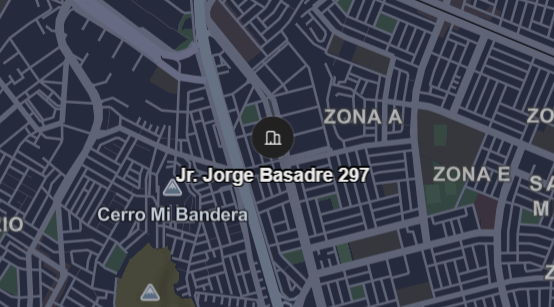
\includegraphics[width=0.55\textwidth]{ubicacion.png}
  
  \label{fig:localizacion}
  \par\footnotesize \textit{Nota.} Elaboración propia a partir de Google Maps (2026)
\end{figure}

\section{Misión, Visión, Objetivo y Valores de la Empresa}

\subsection{Misión}
Diseñar, desarrollar e implementar soluciones informáticas confiables, seguras y adaptadas a las necesidades específicas de las municipalidades peruanas, contribuyendo a la modernización de su gestión administrativa y a la mejora continua de la atención al ciudadano, mediante un servicio técnico cercano y comprometido con cada entidad cliente.

\subsection{Visión}
Consolidarnos, para el año 2030, como la empresa referente a nivel nacional en la estandarización y modernización de los sistemas de gestión municipal, reconocida por la calidad, escalabilidad y sostenibilidad de sus soluciones tecnológicas, y por su aporte a la reducción de la brecha digital entre los gobiernos locales del Perú.

\subsection{Objetivo}
Normalizar progresivamente los sistemas informáticos utilizados por las municipalidades del Perú, reemplazando los desarrollos particularizados y dependientes de infraestructura física o de una sola persona por soluciones web estandarizadas, escalables y de fácil mantenimiento, que optimicen los procesos de gestión municipal y faciliten el acceso a la información para la toma de decisiones.

\subsection{Valores de la Empresa}

\begin{itemize}
  \item \textbf{Compromiso:} con la calidad del servicio brindado a cada municipalidad cliente y con el cumplimiento de los plazos y requerimientos acordados.
  \item \textbf{Confiabilidad:} garantizando la seguridad, disponibilidad e integridad de la información gestionada por los sistemas desarrollados.
  \item \textbf{Innovación:} incorporando de manera constante nuevas tecnologías (como la inteligencia artificial) que aporten valor a la gestión pública local.
  \item \textbf{Responsabilidad social:} entendiendo que las soluciones desarrolladas impactan directamente en la calidad del servicio que las municipalidades ofrecen a los ciudadanos.
  \item \textbf{Adaptabilidad:} ajustando las soluciones tecnológicas a la realidad, presupuesto y capacidad operativa de cada municipalidad atendida.
\end{itemize}

\section{Producto, Mercado y Cliente}

\subsection{Producto}

Consultoría Informática ofrece un sistema integral de gestión municipal orientado al área de rentas y trámites documentarios, que permite automatizar procesos como el registro de contribuyentes y propietarios, la administración del catastro urbano, el procesamiento de transferencias y bajas de propiedades, y la generación de reportes para la toma de decisiones. El producto se entrega actualmente como software de escritorio, aunque se encuentra en proceso de migración hacia una arquitectura web que permita un acceso más flexible y una mejor experiencia de uso para el personal municipal.

\subsection{Mercado}

El mercado objetivo de la empresa está conformado por el sector público local a nivel nacional, específicamente por las municipalidades distritales y provinciales del Perú que requieren digitalizar o modernizar su gestión administrativa. Dado que, según cifras del RENAMU, una parte significativa de los gobiernos locales del país aún no cuenta con sistemas digitales adecuados para sus procesos, este segmento representa un mercado con demanda potencial de crecimiento sostenido, especialmente en municipios distritales de mediana y pequeña escala.

\subsection{Cliente}

Los clientes de Consultoría Informática son las municipalidades peruanas, principalmente aquellas de escala distrital, que requieren soluciones tecnológicas adaptadas a sus procesos internos de gestión de rentas, catastro y trámites documentarios. Entre estos clientes se encuentra actualmente la Municipalidad de San Bartolo, entidad para la cual se desarrolla el presente proyecto de innovación.

\section{Organigrama de la Empresa}

\begin{figure}[H]
  \centering
  \caption{Organigrama de la Empresa}
  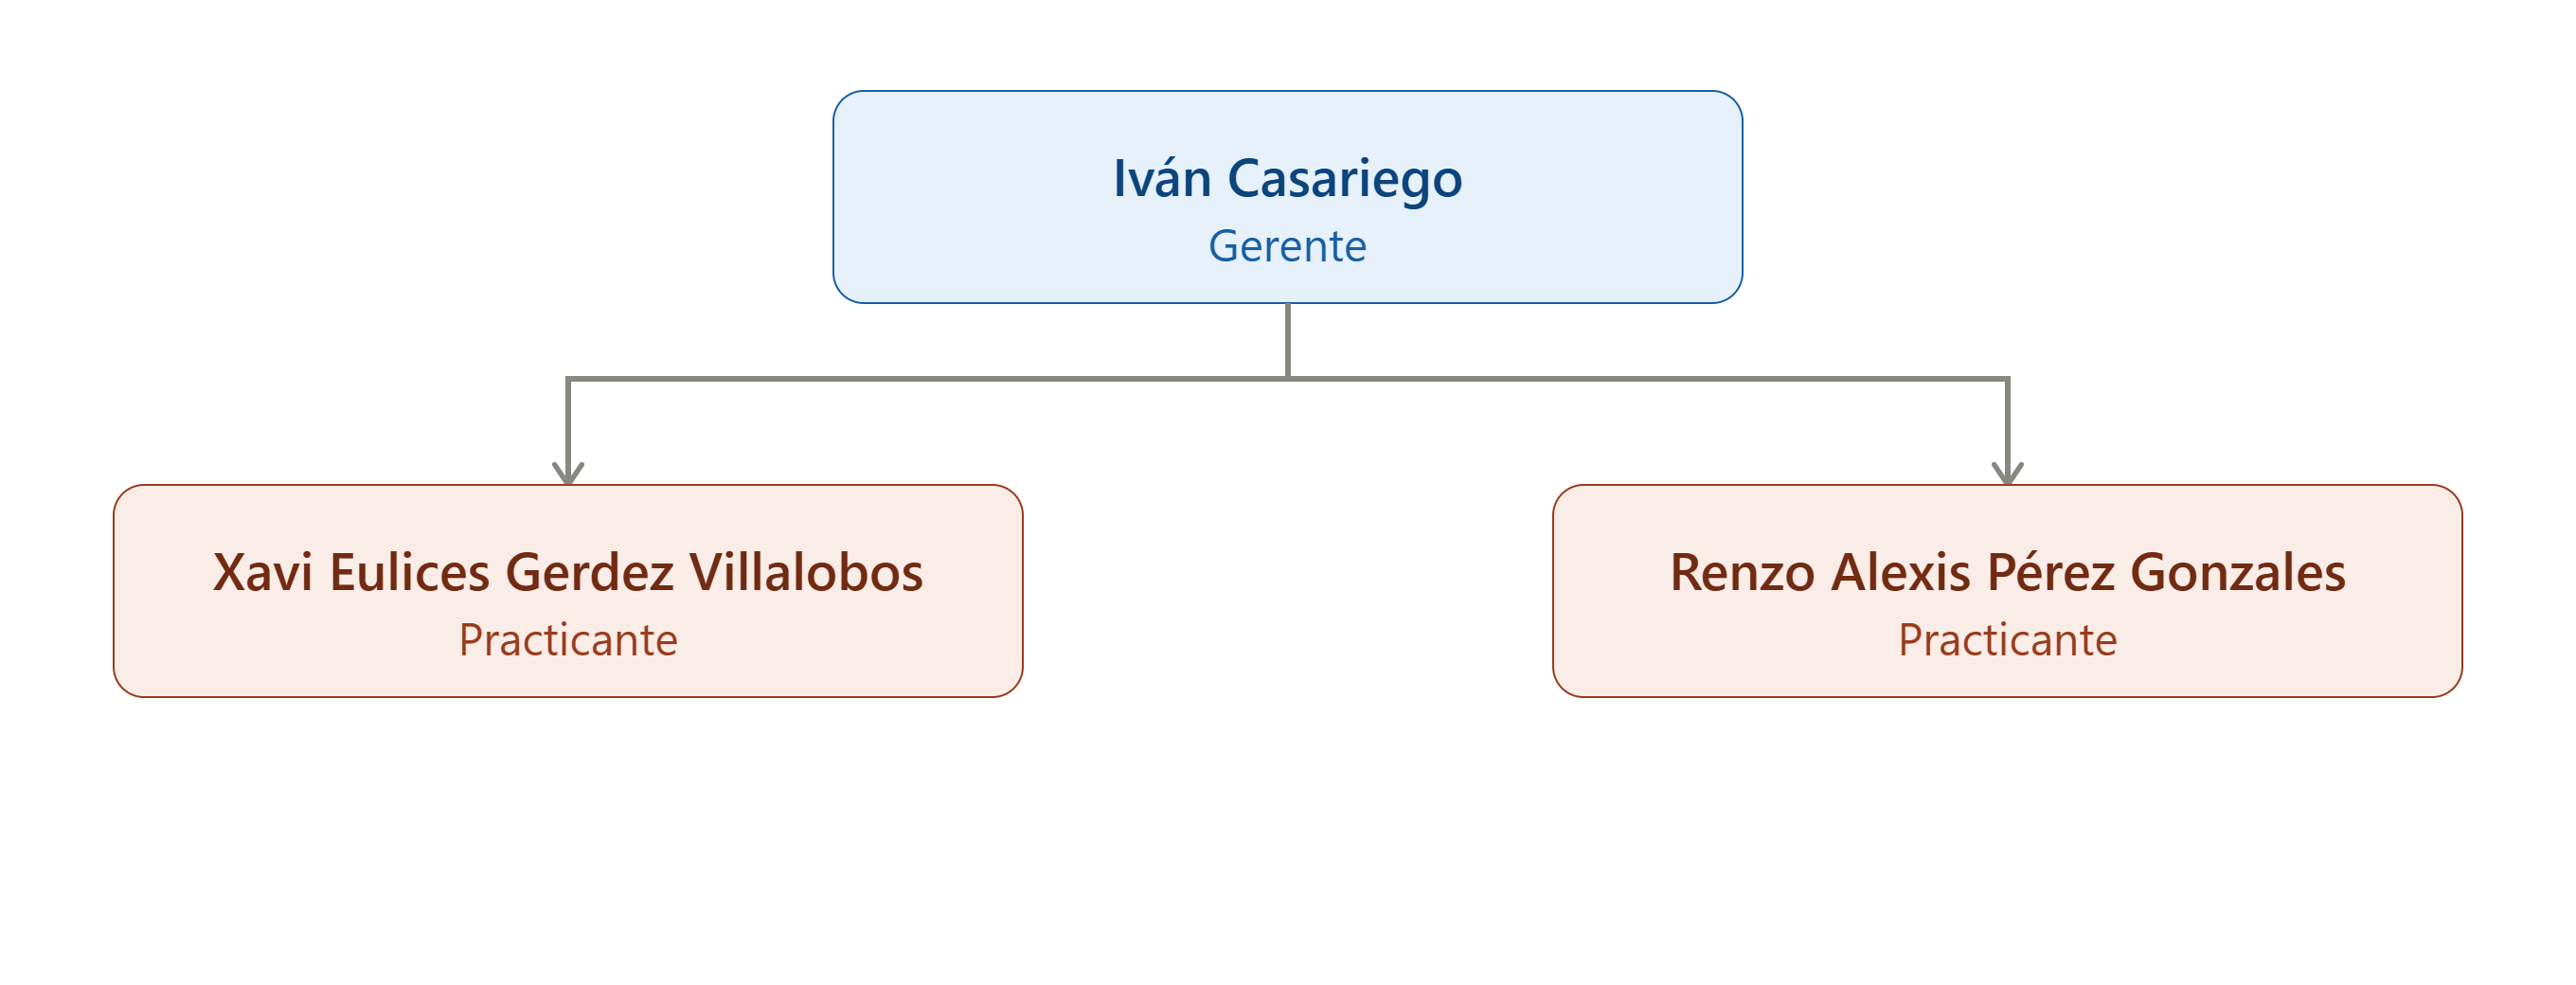
\includegraphics[width=0.9\textwidth]{organigrama.png}
  \label{fig:organigrama}
  \par\footnotesize \textit{Nota.} Se muestra la imagen representativo organizacional con sus jerarquías de la empresa.
\end{figure}

\section{Otra información relevante de la Empresa donde se desarrollará el Proyecto}

\subsection{Planificación y Gestión de la Entrevista}
[Pendiente: aún no se realizó la entrevista con el jefe, coordinador o supervisor del área. Debe incluir fecha y hora, encargado, y las preguntas con sus respuestas reales.]

% CAPÍTULO II: PLAN DE PROYECTO DE INNOVACIÓN / MEJORA / CREATIVIDAD

\chapter{Plan de Proyecto de Innovación / Mejora / Creatividad}

\section{Identificación del Problema Técnico en la Empresa}

\subsection{Problema Local de la Empresa}

Consultoría Informática desarrolla y vende software de gestión a municipalidades, y uno de sus productos es Sispredios, un sistema de gestión tributaria predial desarrollado en Visual FoxPro 9 como aplicación de escritorio. Se trata de un sistema de gran tamaño: el análisis de sus archivos muestra 219 formularios, 202 reportes y 252 tablas en su base de datos principal, que ocupa cerca de 3,5 GB, con alrededor de 1,9 millones de registros en su tabla de cuenta corriente y más de un millón de registros de pagos. % VERIFICAR el significado de la tabla de cuenta corriente al leer el código

Esta tecnología, además, ya no cuenta con respaldo del fabricante: Microsoft mantuvo el soporte extendido de Visual FoxPro hasta enero de 2015 \parencite{taft2007}. A esto se suma que el sistema funciona instalado en equipos locales, por lo que su uso queda limitado a la infraestructura física de cada entidad, y que cada municipalidad atendida cuenta con una solución distinta, construida de manera particular.

Al aplicar el método de Pareto se identificó el problema principal: \textit{falta de estandarización y sostenibilidad en el desarrollo y soporte de los sistemas de software entregados a las municipalidades.} Este problema se origina en cuatro causas. La primera es la \textit{falta de estandarización en los sistemas desarrollados}, ya que cada municipalidad cuenta con una solución distinta, lo que dificulta el mantenimiento, la escalabilidad y la reutilización de código entre proyectos. La segunda son las \textit{interfaces de usuario poco intuitivas, con un diseño UI/UX obsoleto e incómodo}, propio de aplicaciones de escritorio antiguas, que dificulta el uso cotidiano del personal municipal. La tercera son las \textit{demoras en la atención de soporte técnico}, debido a que el conocimiento y la carga de trabajo se concentran en una sola persona y no existen procesos ni personal dedicado exclusivamente a las incidencias, situación que se agrava al depender de una tecnología sin soporte oficial.

La cuarta causa es la \textit{limitación en el acceso a información estadística}: los sistemas actuales no facilitan la generación ni la consulta de reportes consolidados, y el historial de pagos y deudas acumulado durante años no se aprovecha para anticipar la morosidad ni para priorizar la cobranza, por lo que la gestión de cobro se vuelve reactiva. % VERIFICAR con el encargado de la empresa

\subsection{Problema Nacional}

A nivel nacional, la falta de modernización de los sistemas informáticos en las municipalidades del Perú constituye un problema estructural que trasciende a una sola entidad o región. \textcite{francoulco2026} menciona que, según datos del Registro Nacional de Municipalidades (RENAMU) del año 2023, del total de 1,891 municipalidades del país, solo el 47,8\,\% cuenta con Mesa de Partes Virtual, mientras que el 52,2\,\% restante aún no ha implementado este tipo de plataformas digitales. Asimismo, el autor señala que mientras el 86,7\,\% de las municipalidades provinciales ya ha implementado sistemas de este tipo, en el ámbito distrital la adopción se reduce al 43,3\,\% \parencite{francoulco2026}.

Esta brecha se refleja en la gestión tributaria. \textcite{romerocarazas2021} advierten una aparente pasividad fiscal en los gobiernos locales del Perú, que prefieren depender de las transferencias del gobierno central antes que desarrollar nuevas estrategias de recaudación, mientras que \textcite{rojasbarbaran2021} realizaron una revisión sistemática sobre la gestión de la recaudación tributaria en las municipalidades del país. En el caso del impuesto predial, \textcite{riosvelasquez2022} reportan que en la Municipalidad Distrital de El Porvenir (Trujillo) la morosidad de este impuesto era de 72\,\% en 2019 y de 79\,\% en 2020, y que bajó a 65\,\% en 2021 tras aplicar beneficios tributarios en forma de descuentos sobre la deuda.

La falta de herramientas tecnológicas aparece también como un factor del problema. \textcite{soriadiaz2022} describen que en la Municipalidad Distrital de Punchana los contribuyentes deben acudir personalmente a realizar sus trámites porque la entidad no cuenta con servicios en línea y su portal web está desactualizado, y señalan que la ausencia de datos actualizados de los contribuyentes limita el aumento de la recaudación.

En conjunto, estos estudios indican que el problema identificado en Consultoría Informática no es un caso aislado: la desigual capacidad tecnológica de los gobiernos locales y las dificultades de cobranza del impuesto predial son problemas nacionales, lo que abre una oportunidad para que soluciones informáticas estandarizadas, con apoyo de analítica de datos, contribuyan a mejorar la gestión municipal. % TODO: falta 1 artículo científico más (el profesor pidió 5)

\subsection{Problema Internacional}

A nivel internacional, la falta de digitalización y estandarización en la gestión de trámites municipales es una problemática que afecta de manera generalizada a la región latinoamericana, no siendo exclusiva del Perú. \textcite{bid2018} menciona que, en promedio, un ciudadano latinoamericano necesita 5,4 horas para completar una gestión ante una entidad pública, y que el 25\,\% de los trámites requiere tres interacciones o más con la entidad para resolverse, lo cual evidencia la persistencia de procesos burocráticos lentos y poco eficientes en gran parte de los gobiernos de la región.

Asimismo, el organismo señala que el 29\,\% de los ciudadanos de América Latina reportó haber pagado un soborno en el contexto de un servicio público en el último año \parencite{bid2018}, lo que refleja que la ausencia de sistemas digitales estandarizados no solo genera ineficiencia operativa, sino que también favorece espacios de informalidad y corrupción dentro de la administración pública local.

Esta situación confirma que el problema de fondo —sistemas de gestión municipal poco estandarizados, dependientes de procesos manuales o de soluciones tecnológicas aisladas— es una tendencia regional presente en distintos países de Latinoamérica, lo que refuerza la pertinencia de que empresas como Consultoría Informática desarrollen soluciones de software que contribuyan a modernizar y homogeneizar la gestión de los gobiernos locales, no solo en el contexto peruano sino como parte de un desafío compartido a nivel latinoamericano.

\subsection{Formulación del Problema}

\textbf{Problema General}

\medskip
¿De qué forma la implementación de un sistema web de gestión tributaria predial, con un modelo de Machine Learning para estimar el riesgo de morosidad, mejorará la estandarización, el soporte y la sostenibilidad de los sistemas de software que Consultoría Informática brinda a las municipalidades?

\bigskip
\textbf{Problemas Específicos}

\medskip
¿De qué forma la implementación de un sistema web con una arquitectura común y reutilizable (NestJS, React y PostgreSQL) mejorará la estandarización de los sistemas entregados a las municipalidades?

\medskip
¿De qué forma el diseño de una interfaz web moderna, intuitiva y consistente (React y Tailwind CSS) mejorará la experiencia de uso del personal municipal frente a las interfaces obsoletas de escritorio?

\medskip
¿De qué forma un sistema web con una única base de código, desplegada y actualizada de forma centralizada, reducirá las demoras en la atención de soporte técnico?

\medskip
¿De qué forma un modelo de Machine Learning que estime el riesgo de morosidad de los contribuyentes mejorará el acceso a información estadística y la priorización de la cobranza en las municipalidades?

\section{Objetivo del Proyecto de Innovación}

\subsection{Objetivo General}

La implementación de un sistema web de gestión tributaria predial, con un modelo de Machine Learning para estimar el riesgo de morosidad, mejorará la estandarización, el soporte y la sostenibilidad de los sistemas de software que Consultoría Informática brinda a las municipalidades.

\subsection{Objetivo Específico}

\medskip
La implementación de un sistema web con una arquitectura común y reutilizable (NestJS, React y PostgreSQL) mejorará la estandarización de los sistemas entregados a las municipalidades.

\medskip
El diseño de una interfaz web moderna, intuitiva y consistente (React y Tailwind CSS) mejorará la experiencia de uso del personal municipal frente a las interfaces obsoletas de escritorio.

\medskip
Un sistema web con una única base de código, desplegada y actualizada de forma centralizada, reducirá las demoras en la atención de soporte técnico.

\medskip
Un modelo de Machine Learning que estime el riesgo de morosidad de los contribuyentes mejorará el acceso a información estadística y la priorización de la cobranza en las municipalidades.

\section{Antecedentes del Proyecto de Innovación / Mejora / Creatividad (Investigaciones Realizadas)}

\subsection*{Antecedentes Nacionales}
[Pendiente: una tesis nacional sobre predicción de morosidad o aprendizaje automático aplicado a la gestión tributaria municipal.]

\subsection*{Antecedentes Internacionales}
[Pendiente: una tesis internacional sobre modelos de Machine Learning para predecir morosidad o incumplimiento de pago.]

\subsection*{Artículos Científicos}
[Pendiente: artículos científicos sobre Machine Learning aplicado a la recaudación o a la morosidad tributaria.]

\section{Justificación del Proyecto de Innovación / Mejora / Creatividad}

\subsection{Justificación Social}
[Pendiente.]

\subsection{Justificación Legal}
[Pendiente. Normas a verificar antes de citar: Ley de Gobierno Digital (D. Leg. 1412) y Ley 31170 sobre mesas de partes digitales.]

\subsection{Justificación Económica}
[Pendiente.]

\section{Marco Teórico y Conceptual}

\subsection{Fundamento teórico del Proyecto de Innovación / Mejora / Creatividad}

\subsubsection{Sistema Informático}
[Pendiente: definir con libros o artículos, citando con número de página.]

% REFERENCIA BIBLIOGRÁFICA
\printbibliography[title={Referencia Bibliográfica},heading=bibintoc]


% ANEXOS
\chapter*{Anexos}
\addcontentsline{toc}{chapter}{Anexos}

\begin{table}[h]
\centering
\caption{Lista de Problema -- Método de Pareto}
\label{tab:pareto1}
\begin{tabular}{clccccc}
\toprule
\textbf{N°} & \textbf{Identificación del Problema} & \textbf{4 Exc} & \textbf{3 Bue} & \textbf{2 Reg} & \textbf{1 Mal} & \textbf{Total} \\
\midrule
1 & Falta de estandarización & 0 & 1 & 3 & 4 & 13 \\
2 & Demoras en el soporte técnico & 1 & 2 & 3 & 2 & 18 \\
3 & UI/UX obsoleto e incómodo & 0 & 2 & 2 & 4 & 14 \\
4 & Acceso limitado a datos estadísticos & 1 & 3 & 3 & 1 & 20 \\
\bottomrule
\end{tabular}

\vspace{0.3cm}
\footnotesize\textit{Nota.} Elaboración propia, encuesta aplicada a 8 personas colaboradores de la municipalidad.
\end{table}

\begin{table}[h]
\centering
\caption{Lista de Problema -- Método de Pareto (acumulado 80-20)}
\label{tab:pareto2}
\begin{tabular}{clcccc}
\toprule
\textbf{N°} & \textbf{Problemas} & \textbf{N° Enc} & \textbf{\% acum} & \textbf{Frec} & \textbf{80-20} \\
\midrule
1 & Falta de estandarización & 7 & 29.17\% & 29.17\% & Sí \\
2 & UI/UX obsoleto e incómodo & 7 & 58.33\% & 29.17\% & Sí \\
3 & Demoras en el soporte técnico & 6 & 83.33\% & 25.00\% & Sí \\
4 & Acceso limitado a datos estadísticos & 4 & 100\%   & 16.67\% & No \\
\bottomrule
\end{tabular}

\vspace{0.3cm}
\footnotesize\textit{Nota.} Elaboración propia, a partir de la Tabla~\ref{tab:pareto1}.
\end{table}

\begin{figure}[H]
  \centering
  \caption{Diagrama de Pareto}
  \label{fig:pareto}
  \imgopt{0.8}{pareto.png}
  \par\footnotesize\textit{Nota.} Elaboración propia, a partir de la Tabla~\ref{tab:pareto2}, encuesta aplicada a 8 colaboradores de la empresa.
\end{figure}

\end{document}
